%!TEX root = spack-sc15.tex

\subsection{Installation Environment}

Spack is designed to build a consistent HPC stack for our
environment, and reproducible builds are one of our design goals.
Experience at LLNL has shown that reproducing a build manually
is vexingly difficult.
%
Many packages have a profusion of build options. Specifying
them correctly often requires tedious experimentation due to lack of
build standards, as well as the diversity of HPC environments.
For example, in some packages that depend on the {\tt Silo} library,
the \verb|--with-silo| parameter takes a path to {\tt Silo}'s installation 
prefix. In others, it takes the {\tt include} and {\tt lib} subdirectories,
separated by a comma.
The {\tt install} method in Spack's packages encodes precise build
incantations for later reuse.

\subsubsection{Environment isolation}
Inconsistencies arise not only from building manually but also due to 
package installation and user environment differences.
%
For example, LLNL performance tools use two versions of the {\tt libelf}
library. One is distributed with RedHat Linux, while the
other is publicly available. They have the same API but an incompatible ABI.
Specifying the wrong version at build time has caused many
unexpected crashes.

Spack manages the build environment by running each call to {\tt install}
in its own process.  It also sets
{\tt PATH}, {\tt PKG\_CONFIG\_PATH}, {\tt CMAKE\_PREFIX\_PATH}, and
{\tt LD\_LIBRARY\_PATH} to include the dependencies of the current build.
Build systems commonly use these variables to locate dependencies,
and setting them helps to ensure that the correct libraries are detected.
Using a separate process also gives package authors
free reign to set build-specific environment variables without interfering
with other packages.

\subsubsection{Compiler wrappers and RPATHs}
Finding dependencies at build time is not the only obstacle to reproducible
behavior.  As mentioned in Section~\ref{sec:motivation}, binaries must be 
able to find dependency libraries at {\it runtime}.
One of the most common user errors at LLNL is improper library configuration.
Users frequently do not know the libraries with which a package was built, and
constructing a suitable {\tt LD\_LIBRARY\_PATH} for a package that was built 
by someone else is difficult. To reduce the number of support calls that we 
receive, we typically add {\tt RPATHs} to public software installations, so 
that paths to dependencies are embedded in binaries. Thus, users do not need 
to know details of dependencies to run installed software correctly.

Spack manages {\tt RPATHs} and other build policies with
{\it compiler wrappers}.
In each isolated {\tt install} environment, Spack sets the environment variables
{\tt CC}, {\tt CXX}, {\tt F77}, and {\tt FC} to point to its compiler
wrapper scripts.  These variables are used by most build systems to select
C, C++, and Fortran compilers, so they are typically picked up
automatically.\footnote{If builds do not respect {\tt CC}, {\tt CXX}, {\tt FC},
or {\tt F77},
wrappers can be added as arguments or inserted into Makefiles
by {\tt install}.}
When run, the wrappers insert include ({\tt -I}), library ({\tt -L}), and
{\tt RPATH} ({\tt -Wl,-rpath} or similar) flags into the argument list.
These point to the {\tt include} and {\tt lib} directories of dependency
installations, where needed headers and libraries are located.
The wrappers invoke the real compiler with the modified arguments.

Spack's compiler wrappers have several benefits.  First, they allow
Spack to switch compilers transparently in most builds, which is how we
implement compiler options like {\tt \%gcc}.  Second, they enforce the
use of {\tt RPATHs} in installed binaries, which allows applications that 
Spack builds to run correctly {\it regardless of the environment}.  Third, 
because compiler wrappers add header and library search paths for dependencies,
header and library detection tests that most build systems use succeed without
using special arguments for nonstandard locations.  {\tt configure}
commands in Spack's {\tt install} function can have fewer arguments, and can
be written as for system installs, which reduces complexity
for package maintainers and helps to ensure consistent, reproducible
build policies across packages.  Finally, because Spack controls the
wrappers, package authors can programmatically filter the compiler flags
used by build systems, which facilitates porting to bleeding-edge platforms 
or new compilers.

\begin{figure}%{\linewidth}
	\centering
	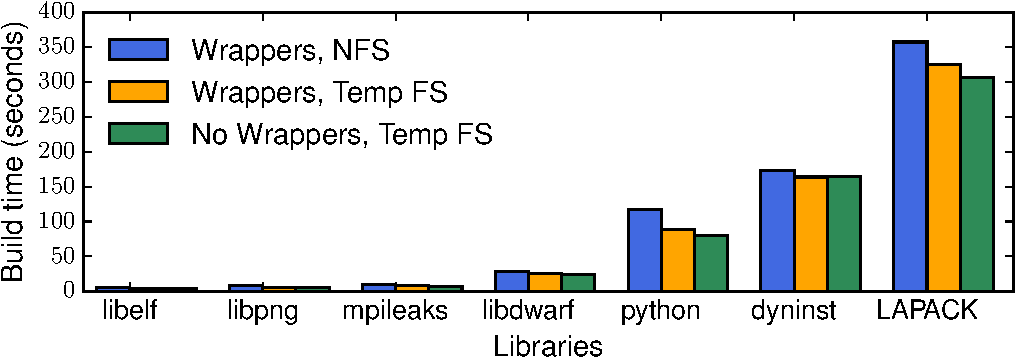
\includegraphics[width=.95\columnwidth]{figs/overhead/build-time.pdf}
	\caption{
		Build time on NFS and temp, with and without wrappers.
		\label{fig:build-times}
	}
\end{figure}
\begin{figure}%{\linewidth}
	\centering
	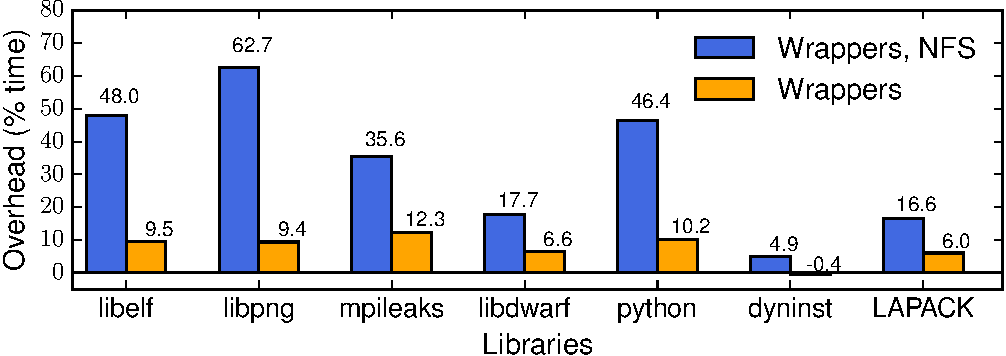
\includegraphics[width=.95\columnwidth]{figs/overhead/overhead.pdf}
	\caption{
		Build overhead of using NFS and compiler wrappers.
		\label{fig:overhead}`
	}
\end{figure}

\subsubsection{Build Overhead}

Argument parsing and indirection cause Spack's compiler wrappers to incur a small
but noticeable performance overhead.  Figure~\ref{fig:build-times} shows
build times with and without compiler wrappers for seven different packages,
and Figure~\ref{fig:overhead} shows the corresponding overhead as a percentage
of the wrapper-less runtime.  {\tt Dyninst} and {\tt LAPACK} use CMake to 
build, and the rest use autotools.  We ran each build three times on an Intel 
Sandy Bridge cluster node, and we report the average. In the case of 
{\tt dyninst}, the overhead is negligible (-0.4\%), but it is as high 
as 12.3\% for shorter builds, like {\tt mpileaks}.

To increase build speed, by default Spack runs each {\tt install} method 
in the default temporary directory, which is a fast, locally-mounted file 
system on most cluster nodes. In our experience, many users build manually 
in their home directories out of habit.  At most sites, home
directories are remotely mounted volumes (e.g., NFS).  To compare Spack builds
with {\it typical} manual builds, we timed the same seven builds using
NFS.  Figure~\ref{fig:overhead} shows that building this way can be as much
as 62.7\% slower than using a temporary file system and
33\% slower on average. We therefore expect many users to notice
a speedup when Spack uses temporary space to build.


\subsubsection{Environment Module Integration}
\label{sec:envmodule}
In addition to managing the build-time environment, Spack can assist in managing
the run-time environment.  A package may need environment variables like {\tt PATH},
{\tt MANPATH}, or {\tt PKG\_CONFIG\_PATH} set before it can be used.
As discussed in Section~\ref{sec:motivation}, many sites rely on environment
modules to setup the runtime environment.  Spack can automatically create simple
dotkit~\cite{dotkit} and Module configuration files for its packages, allowing
users to setup their runtime environment using familiar systems.  While Spack
packages do not need {\tt LD\_LIBRARY\_PATH} to run, we set it in our generated module
files as well, because it can be used by build systems to find libraries, as well
as by dependent packages that do not use {\tt RPATH}.
%
Future versions of Spack may also allow the creation of Lmod~\cite{mclay:lmod}
hierarchies.
%% We discussed Lmod hierarchies generall; we did not discuss using
%% them with Spack so the statment is misleading and unnecessary
%%, as discussed in Section~\ref{sec:env-rpath}.
Spack's rich dependency information would allow automatic generation of 
such hierarchies.
